\documentclass{article}[12pt,titlepage]
\usepackage{graphics,graphicx}
\usepackage{times}
\usepackage{fullpage}
\usepackage{floatflt}
\usepackage{url}
\usepackage{amsmath}
\usepackage{fancyvrb}


% Title Page
\title{{\huge ShapeWorks}\\Particle-based Shape Correspondence and Visualization Software}
\author{Joshua Cates, Manasi Datar, P Thomas Fletcher and Ross Whitaker
\\Scientific Computing and Imaging Institute
\\University of Utah
\\Salt Lake City, USA
\\}

\date{Software Release 0.2.0
\\$Date: 2011/03/28 16:08:52 $
\\$Id: ShapeWorksManual.tex,v 1.9 2011/03/28 16:08:52 wmartin Exp $
\\}

\begin{document}
\maketitle
\begin{center}
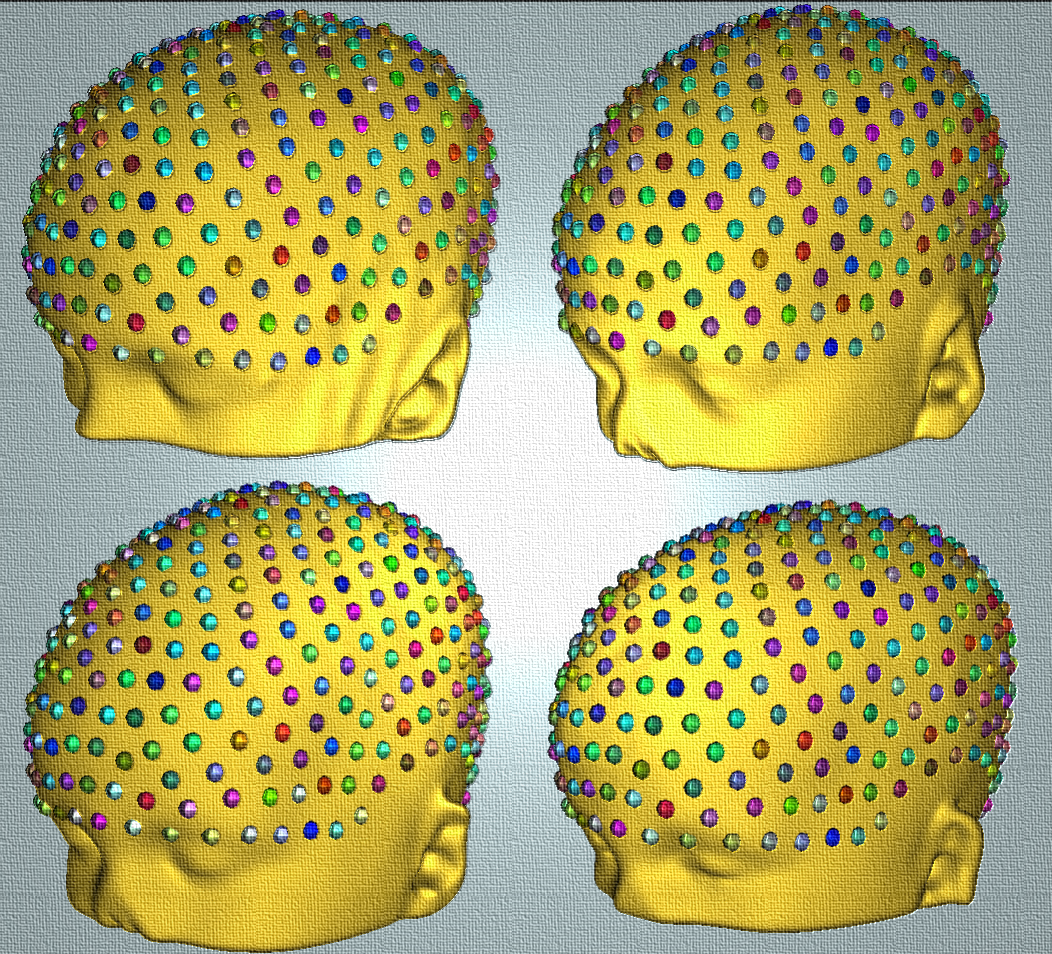
\includegraphics[width=6in]{splashmain.png}
\end{center}
\newpage
\tableofcontents
\newpage

\section{License}
\begin{verbatim}
  For more information, please see: http://software.sci.utah.edu

  The MIT License

  Copyright (c) 2009 Scientific Computing and Imaging Institute,
  University of Utah.


  Permission is hereby granted, free of charge, to any person obtaining a
  copy of this software and associated documentation files (the "Software"),
  to deal in the Software without restriction, including without limitation
  the rights to use, copy, modify, merge, publish, distribute, sublicense,
  and/or sell copies of the Software, and to permit persons to whom the
  Software is furnished to do so, subject to the following conditions:

  The above copyright notice and this permission notice shall be included
  in all copies or substantial portions of the Software.

  THE SOFTWARE IS PROVIDED "AS IS", WITHOUT WARRANTY OF ANY KIND, EXPRESS
  OR IMPLIED, INCLUDING BUT NOT LIMITED TO THE WARRANTIES OF MERCHANTABILITY,
  FITNESS FOR A PARTICULAR PURPOSE AND NONINFRINGEMENT. IN NO EVENT SHALL
  THE AUTHORS OR COPYRIGHT HOLDERS BE LIABLE FOR ANY CLAIM, DAMAGES OR OTHER
  LIABILITY, WHETHER IN AN ACTION OF CONTRACT, TORT OR OTHERWISE, ARISING
  FROM, OUT OF OR IN CONNECTION WITH THE SOFTWARE OR THE USE OR OTHER
  DEALINGS IN THE SOFTWARE.
\end{verbatim}

\section{Introduction} \label{sec:overview}
% insert text from NAMIC Wiki and other papers
This software is an open source distribution of the algorithm for constructing
{\em correspondence-based} statistical models of sets of similar shapes
described by Cates, et al. in \cite{CatesMFCA2006,Cates2007}. Several relevant
extensions to the basic algorithm, as well as their application to clinical and
scientific studies, are also published in
 \cite{Cates2008,CatesMFCA2008,Cates2008,IpekCates2008}.  This document is intended
to provide necessary background information for understanding and using the
ShapeWorks software, including a basic tutorial and reference.  This section
gives a technical overview of correspondence shape models and the
correspondence optimization algorithm that is used in the ShapeWorks software.
For a more detailed explanation of the ShapeWorks optimization algorithm, please
refer to Cates, et al. \cite{Cates2007}.

\subsection{Correspondence Models} 
Correspondence point models represent shape by sampling each shape surface in a
consistently ordered fashion so as to define homologous surface points across
the population of shapes.  These homologous surface points are called {\em
correspondences}.  Once chosen, the 3D positions of all $m$ correspondences on
a shape sample can be encoded as a 3$m$ shape vector, which is the point-based
representation of that shape.  The ordering of the particles on each shape
implies a correspondence among shapes, and the distribution of all of the shape
samples in this 3$m$-dimensional vector space ({\em shape space}) gives rise to
the statistical analysis.  The problem of how to choose the correspondence
positions, and thus the shape-space distribution of the sample population, is a
model selection problem.  Model selection problems in statistics are typically
resolved by choosing the simplest model that explains the observed data (see,
e.g. \cite{Hansen2001}).  Consistent with this idea, the ShapeWorks
correspondence optimization algorithm seeks a compact distribution for its
correspondences in the shape space (for model simplicity), while simultaneously
seeking good surface samplings in order to accurately represent the data.
Figure~\ref{fig:shapespacefig} illustrates these basic concepts for a
population of hand shapes.  The figure shows the mapping of all the surface
point samples from a single shape to a single point in the higher-dimensional
shape space, and the relative compactness of the distribution of all samples in
that shape space after optimization.
\begin{figure}[t]
\centering
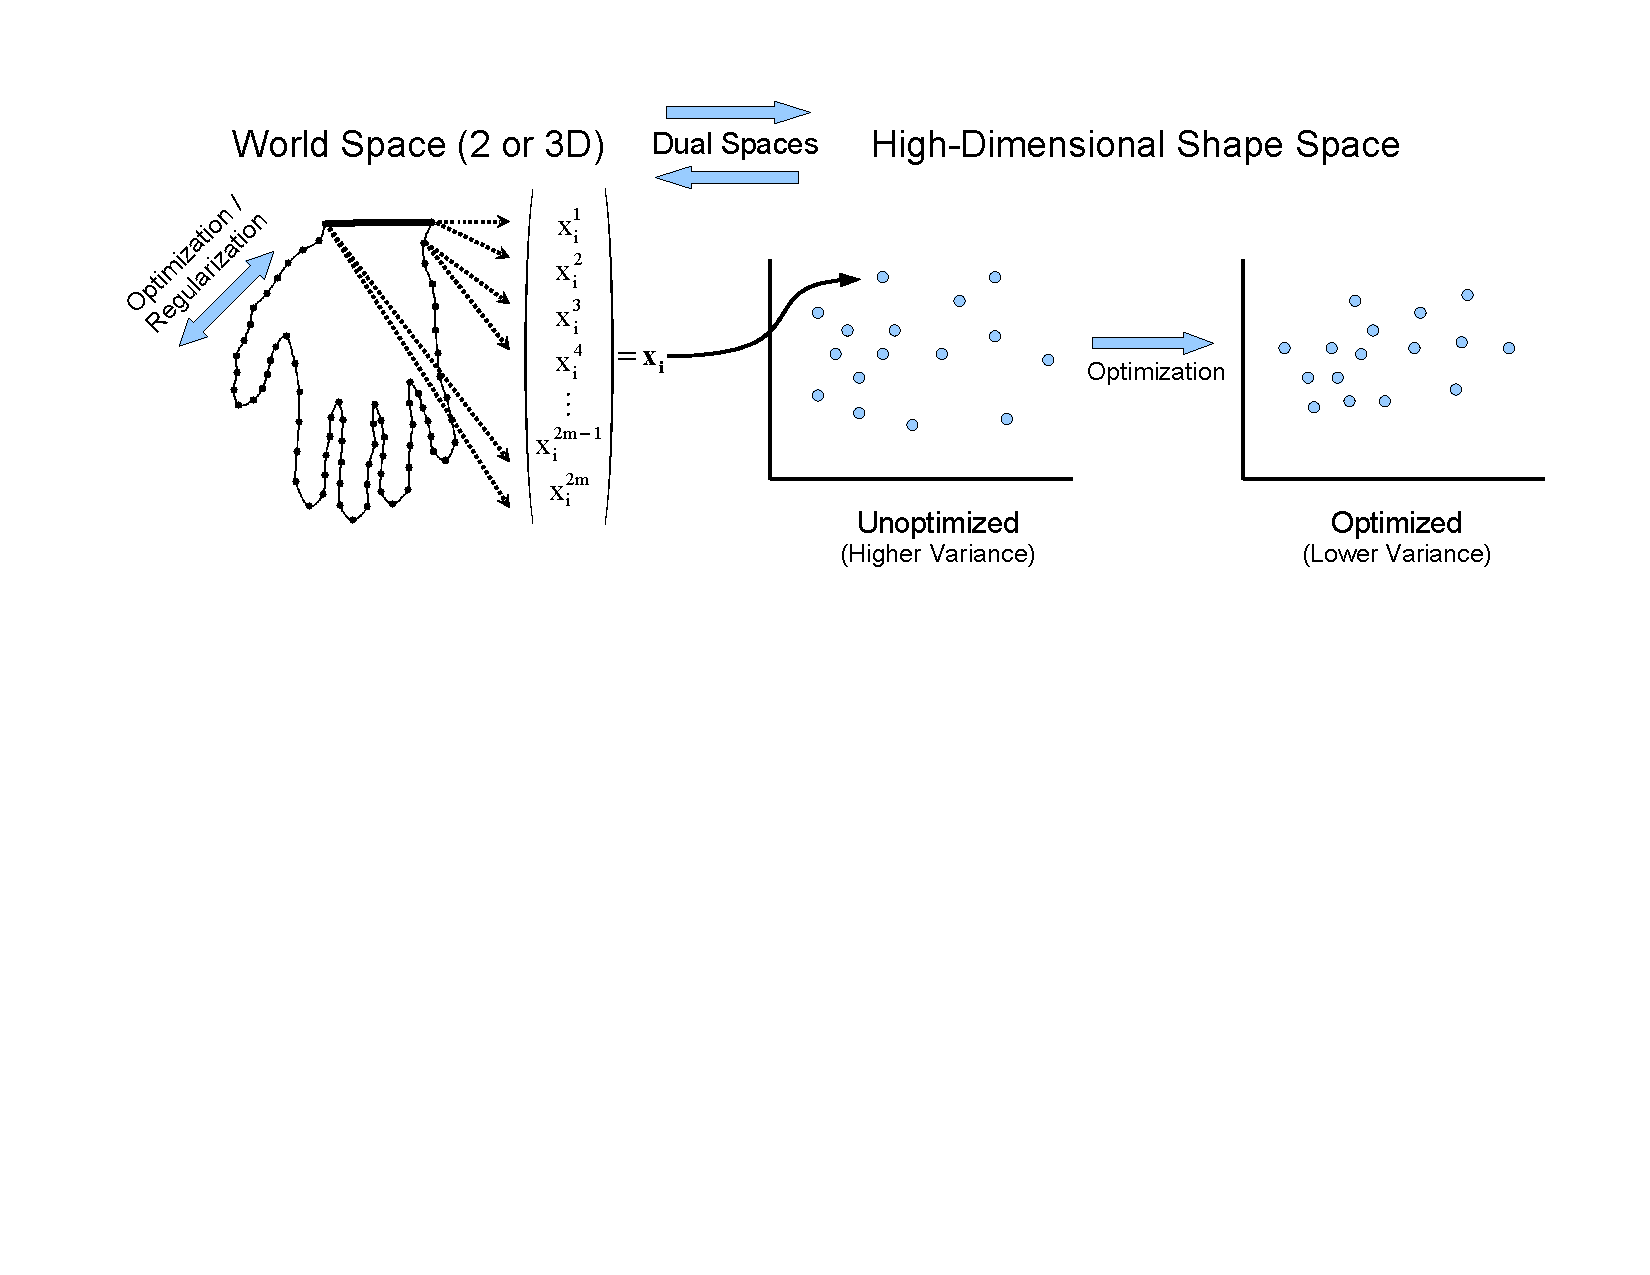
\includegraphics[width=0.9\textwidth]{shapespacefigCropped.pdf}
\caption{An illustration of the basic concepts the ShapeWorks 
point-based correspondence optimization. }
\label{fig:shapespacefig}
\end{figure}

\subsection{The ShapeWorks Correspondence Optimization}
\label{sec:optimization}
The ShapeWorks optimization works by modeling the correspondence positions as
sets of dynamic {\em particles} that are constrained to lie on the set of
sample shape surfaces.  The positions of the correspondences are optimized by
gradient descent on an energy function that balances the negative {\em entropy}
of the distribution of particles on each shape surface with the positive
entropy of the distribution of the shape samples shape space.  More
specifically, and with reference to Figure~\ref{fig:shapespacefig}, we consider
$\mathbf{x}_k \in
\Re^{3m}$ as an instance of a random variable $\mathbf{Z}$ and minimize the
energy function
\begin{equation}
\label{eqn:energyterm}
Q = H(\mathbf{Z}) - \alpha \sum_k H(\mathbf{x}_k),
\end{equation}
where $H$ is an estimation of differential entropy. Minimizing the first term
in $Q$ produces a compact distribution of samples in shape space, while the
second term seeks uniform surface samplings for accurate shape representation.
This latter term can also be modified to adaptively over-sample in response to
local surface features such as curvature. The free parameter $\alpha$ balances
the tradeoff between model compactness and accurate shape representation.
Since correspondence points in this formulation are not tied to a specific
parameterization, the method operates directly on volumetric data and extends
easily to arbitrary shapes, even non-manifold surfaces.

\subsection{The ShapeWorks Shape Modeling Pipeline}
\label{sec:pipeline}
This software distribution consists of several applications that together make
up a full processing pipeline for correspondence computation and visualization.
The stages of the pipeline are as follows,
\begin{equation*}
\mathsf{Preprocessing} \Rightarrow \mathsf{Alignment} \Rightarrow
\mathsf{Initialization} \Rightarrow \mathsf{Optimization} 
\Rightarrow \mathsf{Visualization \& Analysis}
\end{equation*}  
This section gives an overview of the steps involved in the pipeline.  For 
an example of using the ShapeWorks software to perform each of these steps,
see the Tutorial in Section~\ref{sec:tutorial}.

%\paragraph{A Note on Computation Times}
%Processing time on a 2GHz desktop machine scales linearly with the number of
%particles in the system and ranges from 20 minutes for a 2D system of a few
%thousand particles to several hours for a 3D system of tens of thousands of
%particles.

\paragraph{Preprocessing}
Any set of implicitly defined surfaces, such as a set of binary segmentations,
is appropriate as input to this pipeline.  By default, the software will assume
a {\em closed} surface, but can also handle open boundaries (specified by
cutting planes) and non-manifold surfaces consisting of multiple closed
surfaces.  A binary mask, such as the output of an image segmentation process,
for example, contains an implicit shape surface at the interface of the labeled
pixels and the background. Binary masks contain aliasing artifacts, however,
that should first be removed. %We have found that the
%$r$-tightening algorithm given by Williams et al. \cite{Williams2005} is
%effective in removing these artifacts without compromising the precision of the
%segmentation.  
Typically we follow an antialiasing step with a very slight
Gaussian blurring to remove the high-frequency artifacts that can occur as a
result of numerical approximations.

\paragraph{Alignment}
A collection of shape segmentations must often be aligned in a common
coordinate frame for modeling and analysis.  The ShapeWorks software does not
provide full support for this stage of the pipeline, since every new dataset
may require a different process of alignment.  Some basic alignment tools that
are included with ShapeWorks are the ability to align the segmentations
with respect to their centers of mass and the orientation of their first
principal eigenvectors.  For some classes of data, this method is effective as
a rough alignment and is followed, {\em during the optimization process}, by
iterative Procrustes alignments based on the correspondence point positions
 \cite{Goodall91}.  For more information on this procedure, see 
Sections~\ref{sec:tutorial} and \ref{sec:reference}.

The ShapeWorks software distinguishes between two separate coordinate frames: 
a {\em local} coordinate frame for each shape sample, and a {\em common} 
coordinate frame in which all shape samples are coregistered.  For applications
in which the input data is completely registered, these two coordinate frames
are the same.   Where there is a distinction, the ShapeWorks software will
maintain and output appropriate transformations to the common coordinate frame
for each shape sample, as well as separate correspondence files for each coordinate
frame.

\paragraph{Correspondence Initialization}
Typically, we initialize the ShapeWorks optimization with a single particle that
finds the nearest zero of the implicit surface, and then splits under
optimization (producing a new, nearby particle) at regular intervals until a
specific number of particles are produced and reach a steady state.  This
initialization procedure is supported with the ShapeWorks software. We have
found this procedure to be generally applicable to classes of closed shapes
with reasonably smooth surfaces.  For more complicated shapes, it may be
necessary to specify initial particle positions for the optimization
using other means.  Initial particle positions may be computed offline and
supplied to ShapeWorks as a text file input (see Section~\ref{sec:fileformats}).

\paragraph{Correspondence Optimization}
The ShapeWorks optimization proceeds as described in
Section~\ref{sec:optimization}, starting with an initial set of particle
positions and a set of implicit surfaces (e.g. distance transforms).
Several types of optimization procedures are supported:
adaptive gradient descent, Jacobi updates, and Gauss-Seidel updates.  By
default, adaptive gradient descent with Gauss-Seidel updates is used.
Important parameters to consider for the optimization are the regularization on the covariance matrix for the
shape-space entropy estimation, and the parameter $\alpha$ from
Equation~\ref{eqn:energyterm} which controls the trade-off between the
uniformity of the surface sampling and the compactness of the optimized model.
Also consider whether iterative Procrustes alignment is necessary and whether
or not to remove Procrustes {\em scale} from the correspondence model.

%\paragraph{Adaptive Surface Sampling}

%\paragraph{Cutting Planes}

\paragraph{Visualization and Analysis}
Statistical analysis of point-based shape models is difficult because
point-wise statistical tests require multiple-comparisons corrections that
significantly reduce statistical power \cite{CatesMFCA2008}. Analysis in the full shape space,
however, is problematic due to the high number of dimensions and the difficulty
of obtaining sufficient samples. A common solution is to employ dimensionality
reduction reduction by choosing a subspace in which to project the data for
traditional multivariate analysis (see, e.g. \cite{CatesMFCA2008,CatesMICCAI2008}).

This software does {\em not} include specific code for statistical analysis of
the correspondences.  It does, however, provide principal component analysis
(PCA), which can be used for dimensionality reduction prior to subsequent
statistical analysis, and visualization of orthogonal modes of variation in the
model (see, e.g. \cite{CatesMFCA2008,CatesMICCAI2008}.  ShapeWorks also includes
methods for computing and visualizing the Euclidean mean shapes and the median
shapes of populations.  Typically, we use a separate statistical package, such
as {\em R} (the R Foundation, \texttt{www.r-project.org}), for analysis of the
PCA loadings of the correspondence positions.  For more ideas regarding 
visualization and statistical analysis of correspondence models, see the
various publications listed in the bibliography section of this document.

%For our multivariate metric of shape, we
%propose to use a standard, data-driven approach to dimensionality reduction and
%project the correspondences into a lower dimensional space determined by
%choosing a number of basis vectors from principal component analysis
%(PCA). Ideally, we would like to choose only PCA modes that account for
%variance that cannot be explained by random noise.

%To visualize group differences that are driving the statistical result, we
%compute the linear discriminant vector implicit in the Hotelling T2 statistic,
%which is the is the line along which the between-class variance is maximized
%with respect to the within-class variance (Fisher�s linear discriminant). The
%discriminant vector can be rotated back from PCA space into the full
%dimensional shape space, and then mapped onto the mean group shape
%visualizations to give an indication of the significant morphological
%differences between groups.

%To visualize deformations between the group mean shapes, we can compute metrics
%on the displacement field describing the mapping from points $x$ on one group
%mean to corresponding points $x_0$ on the another. Using the set of
%correspondence points, a smooth transformation $T(x) = x_0$, can be computed
%using a thin-plate spline interpolation. We propose to visualize strain, a
%measure on the Jacobian of the deformation field $x-T(x)$ that describes the
%local stretching and compression caused by the deformation. An effective
%visualization for the strain tensor is an ellipsoid with principal axes given
%by the principal directions and magnitude of strain.

\section{The ShapeWorks Software}
This section provides an overview of how to build and use the ShapeWorks
software. The tutorial in this section illustrates a full shape analysis
pipeline, starting with binary volume segmentations, and including
preprocessing and visualization of correspondences.  For more detailed software
usage information, see Section~\ref{sec:reference}.

\subsection{Overview of the Executables}
\paragraph{ShapeWorksGroom} This is a command-line preprocessing tool for image volumes.  Its
primary purpose is to convert binary, volumetric image segmentations (label
masks) into distance transforms that are suitable for input to the ShapeWorksRun and
ShapeWorksShop applications.  Filtering operations are implemented using ITK
(The Insight Toolkit), and are applied in batch processing mode.  Some of the
filtering operations that ShapeWorksGroom supports are antialiasing, automatic
cropping, hole-filling, smoothing, and distance transforms.

\paragraph{ShapeWorksRun}  This is the command-line correspondence optimization tool, and the
heart of the ShapeWorks shape analysis pipeline.  The minimum required input to
this application is a set of distance transforms that are the surface
representations of the population of shapes (see Sec.~\ref{sec:pipeline}).
Intial particle positions and affine registration information can also be
supplied as inputs.  ShapeWorksRun can be used to initialize a set of particle
positions using the particle-splitting described Sec.~\ref{sec:pipeline} .

\paragraph{ShapeWorksView}  This tool can be used to visualize optimized correspondence 
positions, along with surface reconstructions based on the correspondences. It also computes
a principal component analysis (PCA) of the correspondences, and allows you to visualize
the variation in each of the modes of the PCA.  The mean shapes and the median shapes can 
be reconstructed, and ShapeWorksView allows you to assign group labels to your samples, 
in order to visualize the differences in mean shape between the groups.

\paragraph{ShapeWorksShop}  This is a GUI-based version of ShapeWorksRun that has some 
additional functionality and optimization parameters exposed.  It provides a
real-time visualization of the optimation process on the set of shape surfaces.
This tool is very useful, for example, for initializing a set of particles
prior to the full optimization and for testing parameter settings.

\subsection{File Formats}
\label{sec:fileformats}
%\subsection{Inputs and Outputs (File Formats)}
\paragraph{Image volumes} Inputs to ShapeWorksGroom, ShapeWorksRun, and ShapeWorksShop are 
image volumes.  ShapeWorks can read and write any image file format supported by
the Insight Toolkit.  Image inputs to ShapeWorksRun and ShapeWorksShop must be
surfaces embedded in image volumes.  Shape surfaces must be represented
implicitly as the zero level set of a distance transform.

\paragraph{Point files} Correspondence point positions are stored in text files.  These files contain
no header, and are simply a list of the point positions written as follows\\
\texttt{x1 y1 z1\\x2 y2 z2\\ \vdots\\xN yN zN },\\
where \texttt{x y z} are floating point numbers and \texttt{N} is the number of correspondence points.
Two point files are maintained for each shape.  The first has file extension \texttt{.lpts}, and is the
correspondence positions in that shape's {\em local} coordinate space.  The second file has extension
\texttt{.wpts}, and is the correspondence positions in the {\em common} (world) coordinate space.  
The \texttt{.lpts} files can be used to initialize particles on shape surfaces for optimization, while the
\texttt{.wpts} files should be used for any statistical analysis.

%\paragraph{Transform files} Need description here.
\paragraph{Parameter files} ShapeWorks software parameters are specified in text files.  The syntax for 
these parameter files is described in Section~\ref{sec:params}.

\subsection{Building the Software}
\paragraph{Dependencies}
The ShapeWorks software depends on several open-source, freely-available
software toolkits.  To build the full set of tools, including the graphical
interfaces, you will need the following packages.
\begin{description}
\item[\textbf{CMake}] is used to configure the build, and is available 
from \verb+http://www.cmake.org+.  The SCMoguls build is compatible with CMake
2.6.  Earlier versions of CMake may not be supported.
\item[\textbf{The Insight Toolkit (ITK)}] is required for all ShapeWorks applications.  ITK is available 
from \verb+http://www.itk.org+.  Make sure to use ITK version 2.8.1 or higher.
For compatibility with ShapeWorks, build ITK using CMake and compile in {\em
Release} mode.
\item[\textbf{The VisualizationToolkit (VTK)}] is required only for ShapeWorksView and ShapeWorksShop.  VTK is
available from \verb+http://www.itk.org+.  ShapeWorks has been tested with VTK
version 5.0 and higher.  For compatibility with ShapeWorks, build VTK using
CMake and compile in {\em Release} mode.
\item[\textbf{Fast Light Toolkit (FTLK)}] is required for ShapeWorksView and ShapeWorksShop.  FLTK is
available from \\ \verb+http://www.fltk.org+.  The most recent stable release of
FLTK version 1.1.x is recommended. For compatibility with ShapeWorks, build FLTK
using CMake and compile in {\em Release} mode.
\end{description}

\paragraph{Supported Platforms}
The ShapeWorks software is ANSI C++ code and has been built successfully on
Windows 32-bit, Linux 32-bit, and Linux 64-bit platforms.  Any platform for
which ITK, VTK, and FLTK are supported should, in theory, also support the
ShapeWorks software.

\paragraph{Binary Distributions}
Binary distributions of the ShapeWorks software for Windows 32-bit platforms are
also available for download.  Binaries for other platforms (e.g. Macintosh and
Windows 64-bit) may be released in the future.  Unless you intend to do
development with the ShapeWorks source code, it is highly recommended that you
use a binary distribution, if one is available for your system.

\paragraph{Support}
Questions regarding the ShapeWorks software can be addressed to the ShapeWorks
mailing list at \\ \texttt{shapeworks-users@gforge.sci.utah.edu}.  You can sign
up for this mailing list by visiting
\\ \texttt{https://gforge.sci.utah.edu/mailman/listinfo/shapeworks-users}.\\
You can visit the ShapeWorks discussion forums, and browse news and development
information at the ShapeWorks GForge page
\\ \texttt{https://gforge.sci.utah.edu/gf/project/shapeworks/}.

\paragraph{Build Instructions}
ShapeWorks uses the CMake build system to configure the build and generate
makefiles or Microsoft Project files.  Once configured, ShapeWorks can be built
with your platform's native compiler (gcc, Microsoft C++, etc).  The following
configure instructions are the same for every platform.  For more information
on using CMake, please refer to www.cmake.org.
\begin{enumerate}
\item Unzip or untar the source code distribution.  
\item Create a separate build directory for your ShapeWorks build files and exectuables.
If your source code is in \texttt{/home/username/ShapeWorks}, for example, you
might choose to create a directory \\ \texttt{/home/username/ShapeWorks\_build}.  On
linux/unix platforms, you will need a build for each compilation configuration,
e.g. you might have two build directories:
\texttt{/home/username/ShapeWorks\_release} and
\texttt{/home/username/ShapeWorks\_debug}.  Note that you will also need
corresponding {\em Debug} and {\em Release} builds for ITK, VTK, and FLTK.
\item Start the CMake GUI, or run \verb+ccmake+ if building from a terminal shell.  
\item Enter the \texttt{ShapeWorks/code} directory as your source code directory and your
newly-created directory as the build directory.
\item In the CMake GUI, choose ``Configure''.  CMake will attempt to find your ITK build. 
If not found, you will need to specify the {\em build} directory for ITK.
\item In the CMake GUI, you will have the option to choose to build the ShapeWorksView and
ShapeWorksShop applications.  If selected, CMake will attempt to
automatically configure FLTK and VTK.  If these builds are not found, you will
need to specify their locations.
\item Specify the \texttt{CMAKE\_INSTALL\_PREFIX}.  This is the directory in which the executables
will be installed.
\item On Linux/Unix systems, specify {\em Release} mode for your build.  If you also want
a developmental build, you will need to configure a separate build directory
for a {\em Debug} mode.  On Windows platforms, you may choose either Debug or
Release at compile time.
\item Once ITK, VTK, and FLTK are properly configured, click ``Generate'' to create the 
makefiles.
\item Build the {\em INSTALL} target in the CMake-generated makefiles using 
your native compiler.
\item[\large\textbf{!}] Important: Make sure to build using {\em Release} mode for best results.  
Because ShapeWorks and ITK both rely heavily on compile-time optimizations, if
built using a {\em Debug} configuration, SCIRunMoguls code may run up to ten
times slower!
\end{enumerate}

\section{Tutorial: Torus Example}
\label{sec:tutorial}
% describe data
This tutorial will illustrate how to use the ShapeWorksRun software to optimize
correspondences on image segmentations (i.e., binary volumes), which are a
common format in many shape studies that rely on 3D imaging to extract anatomy.
In this example, we will compute a statistical model of $20$ synthetically
generated tori.  The tori are parameterized by small radii $r$ and a large
radii $R$, each randomly sampled from a Gaussian distribution.  The resulting
shape model will therefore show two orthogonal modes, with the variance in each
of these modes corresponding to that of the sampled distributions for $r$ and
$R$.  This tutorial proceeds step-by-step through the full analysis pipeline
described in Section~\ref{sec:pipeline}. An example of $7$ synthetically generated misaligned "mickey" datasets
is also provided to illustrate how iterative closest point (ICP) registration can be used to improve the alignment in ShapeWorksGroom (ShapeWorks/example directory).
%, which also provides references to any
%relevant publications.

%\begin{enumerate}
%\item \textbf{The Torus Data.}
\subsection{The Torus Data}
The example set of torus shapes is provided in the \texttt{ShapeWorks/examples} directory.
Navigate to this directory and unzip the \texttt{TorusExample.tgz/.zip} data file.  You
should now have a new directory, \\ \texttt{ShapeWorks/examples/TorusExample}, which
contains $20$ synthetically generated tori, The tori are represented as binary
volumes, i.e. as image segmentations.  Pixels inside each torus have value $1$,
and pixels outside have value $0$.

%\item \textbf{Preprocessing.}
\subsection{Preprocessing with ShapeWorksGroom}
As discussed in Section~\ref{sec:pipeline}, the first step is to convert the
binary volume into a distance transform suitable for use with ShapeWorksRun.  We
will do this using ShapeWorksGroom to perform a set of filtering operations.
The first preprocessing step is to crop all of the image volumes to the same
size, and shift the center of each volume to the center-of-mass of the
segmentations.  This establishes a common coordinate frame, an initial, rough
translational alignment, and a common image volume size.  This latter
consideration is highly recommended when using ShapeWorksRun.  Note that if the
shapes embedded in your own image volumes are already in alignment, then these
operations are not needed.  (In the case of the torus data, this step is also
not necessary, but is illustrated here because it may be generally useful for
real-world data.)  Before cropping, we will also perform morphological
operations to isolate the foreground and fill any existing holes in the
segmentations.

From the example directory, type the following command. Note that you may need
to also specify a path to the executables if they are not already in your
system path. This preprocessing step should take less than 5 minutes to run,
depending on the speed of your computer.  The parameter file for this step is
shown in Figure~\ref{fig:preprocessing1}, and contains all of the required parameters
for each stage of processing.
\begin{Verbatim}[frame=single]
ShapeWorksGroom torus.preprocess1.params isolate hole_fill center auto_crop
\end{Verbatim}
\begin{figure}[t]
\centering
\begin{Verbatim}[fontsize=\small,frame=single,framerule=1mm]
// torus.preprocess1.params
// Preprocessing parameters 1 for Torus example
(background 0.0) // Value of background pixels in the image
(foreground 1.0) // Value of foreground pixels in the image
(pad 10)         // Number of background pixels to pad the edges of
                 // the cropped volume

(verbose 1)      // Output progress information

(inputs          // Set of input files to process
"torus.00.mha"  "torus.01.mha"  "torus.02.mha"  "torus.03.mha"
"torus.04.mha"  "torus.05.mha"  "torus.06.mha"  "torus.07.mha"
"torus.08.mha"  "torus.09.mha"  "torus.10.mha"  "torus.11.mha"
"torus.12.mha"  "torus.13.mha"  "torus.14.mha"  "torus.15.mha"
"torus.16.mha"  "torus.17.mha"  "torus.18.mha"  "torus.19.mha"
)

(outputs            // Output filenames to use
"torusDT.00.mha"  "torusDT.01.mha"  "torusDT.02.mha"  "torusDT.03.mha"
"torusDT.04.mha"  "torusDT.05.mha"  "torusDT.06.mha"  "torusDT.07.mha"
"torusDT.08.mha"  "torusDT.09.mha"  "torusDT.10.mha"  "torusDT.11.mha"
"torusDT.12.mha"  "torusDT.13.mha"  "torusDT.14.mha"  "torusDT.15.mha"
"torusDT.16.mha"  "torusDT.17.mha"  "torusDT.18.mha"  "torusDT.19.mha"
)
\end{Verbatim}
\caption{\label{fig:preprocessing1}Parameter file for the first stage of torus preprocessing
with ShapeWorksGroom: foreground isolation,
hole-filling, and automatic volume cropping.}
\end{figure}

\begin{figure}
\centering
\begin{Verbatim}[fontsize=\small,frame=single,framerule=1mm]
// torus.preprocess2.params
// Preprocessing parameters 2 for Torus example

(background 0.0) // Value of background pixels in image
(foreground 1.0) // Value of foreground pixels in image
(antialias_iterations 20) // Number of anti-aliasing iterations
(blur_sigma 2.0) // Size of Gaussian blurring kernel for smoothing
(fastmarching_isovalue 0.0)  // Pixel value associated with shape surfaces

(inputs                         // Name of input files
"torusDT.00.mha" "torusDT.01.mha" "torusDT.02.mha" "torusDT.03.mha"
"torusDT.04.mha" "torusDT.05.mha" "torusDT.06.mha" "torusDT.07.mha"
"torusDT.08.mha" "torusDT.09.mha" "torusDT.10.mha" "torusDT.11.mha"
"torusDT.12.mha" "torusDT.13.mha" "torusDT.14.mha" "torusDT.15.mha"
"torusDT.16.mha" "torusDT.17.mha" "torusDT.18.mha" "torusDT.19.mha"
)

(outputs                        // Name of output files
"torusDT.00.mha" "torusDT.01.mha" "torusDT.02.mha" "torusDT.03.mha"
"torusDT.04.mha" "torusDT.05.mha" "torusDT.06.mha" "torusDT.07.mha"
"torusDT.08.mha" "torusDT.09.mha" "torusDT.10.mha" "torusDT.11.mha"
"torusDT.12.mha" "torusDT.13.mha" "torusDT.14.mha" "torusDT.15.mha"
"torusDT.16.mha" "torusDT.17.mha" "torusDT.18.mha" "torusDT.19.mha"
)
\end{Verbatim}
\caption{\label{fig:preprocessing2}Parameter file for the second stage of torus preprocessing
with ShapeWorksGroom: antialiasing,
distance transform computation, and slight blurring.}
\end{figure}

The second preprocessing step antialiases the binary surface, and then computes
a distance transform from that surface using the fastmarching method.  Finally,
we blur the distance transform slightly to get rid of high-frequency artifacts.
Type the following command.  This step should also take less than 5 minutes to 
complete.  The parameter file for this step is given in Figure~\ref{fig:preprocessing2}.
Type the following command.
\begin{Verbatim}[frame=single]
ShapeWorksGroom torus.preprocess2.params antialias fastmarching blur
\end{Verbatim}
At this stage, you should have a set of implicit surface volumes labeled
\texttt{torusDT.00.mha, torusDT.01.mha, ..., torusDT.19.mha}.  These new
files are suitable inputs to the correspondence optimization.

%\item \textbf{Optimization.}
\subsection{Optimizing Correspondence with ShapeWorksRun}
% particle system commands, parameter files
The next step is to initialize and optimize the particle system.  In this
example, we will use relatively few points, just 256 particles per
torus. Correspondences are initialized on the shape surfaces using the
splitting strategy described in Section~\ref{sec:pipeline}, and optimized using
Gauss-Seidel adaptive gradient descent on the minimum-entropy algorithm from
Section~\ref{sec:optimization}.  We will save the progress of the optimization
every 20 iterations by setting the checkpointing option.  A full parameter file
for this step is shown in Figure~\ref{fig:correspondence}.  The command to 
start the optimization is as follows.
\begin{Verbatim}[frame=single]
ShapeWorksRun torus.correspondence.params
\end{Verbatim}
\begin{figure}
\centering
\begin{Verbatim}[fontsize=\small,frame=single,framerule=1mm]
// torus.correspondence.params
// Parameters for the correspondence point optimization with ShapeWorksRun 
// (or ShapeWorksShop)
(inputs  // List of files containing the set of shape surfaces (distance transforms)
"torusDT.00.mha" "torusDT.01.mha" "torusDT.02.mha" "torusDT.03.mha"
"torusDT.04.mha" "torusDT.05.mha" "torusDT.06.mha" "torusDT.07.mha"
"torusDT.08.mha" "torusDT.09.mha" "torusDT.10.mha" "torusDT.11.mha"
"torusDT.12.mha" "torusDT.13.mha" "torusDT.14.mha" "torusDT.15.mha"
"torusDT.16.mha" "torusDT.17.mha" "torusDT.18.mha" "torusDT.19.mha"
)

// OPTIONALLY we could specify a set of point files to initialize
// the optimization like this:
// (point_files torusDT.00.lpts torusDT.01.lpts ... torusDT.19.lpts)

(number_of_particles 256) // If point files are not specified, then
                          // the application will initialize particles
                          // by splitting until each shape has this 
                          // total number of particles.

(iterations_per_split 200) // Iterations between splitting during
                          // initialization phase.

(starting_regularization 10.0) // Starting regularization for the
                                // entropy-based correspondence
                                // optimization.

(ending_regularization 0.1) // Final regularization for the entropy-
                            // based correspondence.

(optimization_iterations 200) // Number of iterations for the entropy-
                              // based correspondence.

(checkpointing_interval 20) // Number of iterations between checkpoints
                            // (iterations at which results are saved)

(output_points_prefix "torus") // Prefix for the output files.
\end{Verbatim}
\caption{\label{fig:correspondence}Parameter file for the correspondence point optimization
of the torus data using ShapeWorksRun.}
\end{figure}
During the optimization, ShapeWorksRun outputs the variance associated with each
of the orthogonal modes of variation in the data, obtained via principal
component analysis (PCA).  As the optimization proceeds, notice how almost all of the
variation in the model is shifted into the top two modes of variation (modes 18
and 19).  These two modes represent our two real parameters of the model, big
$R$ and little $r$.  The initialization and optimization process will take between
5 to 10 minutes, depending on the speed of your computer.  In practice, you will need
to modify the regularization parameter and the number of iterations for your data.  In
general, real data will require more particles per shape and more iterations for a better
model fit.  Also consider setting the \texttt{adaptivity\_strength} parameter to 
introduce oversampling in regions of higher curvature.  The \texttt{relative\_weighting}
parameter, which sets $\alpha$ from Equation~\ref{eqn:energyterm}, may also 
be of interest.  By default, $\alpha$ is set to $1$.

\subsection{Visualization and Analysis with ShapeWorksView}
We will now use the ShapeWorksView application to view the output of the correspondence
optimization.  Note that you can also view the intermediate results of the optimization
after each checkpointing save.  First, start the ShapeWorksView application using the
supplied parameter file, as given in Figure~\ref{fig:visualization}.  Note that this
parameter file load the \texttt{*.wpts} files, which are the correspondences
in the common (world) coordinate space.  To start the ShapeWorksView application, type the
following command.
\begin{Verbatim}[frame=single]
ShapeWorksView torus.analyze.params
\end{Verbatim}
\begin{figure}
\centering
\begin{Verbatim}[fontsize=\small,frame=single,framerule=1mm]
// torus.analyze.params
// Parameters for viewing correspondence points using ShapeWorksView
(point_files    // Set of correspondence points in the common coordinate space.
"torus.00.wpts" "torus.01.wpts" "torus.02.wpts" "torus.03.wpts"
"torus.04.wpts" "torus.05.wpts" "torus.06.wpts" "torus.07.wpts"
"torus.08.wpts" "torus.09.wpts" "torus.10.wpts" "torus.11.wpts"
"torus.12.wpts" "torus.13.wpts" "torus.14.wpts" "torus.15.wpts"
"torus.16.wpts" "torus.17.wpts" "torus.18.wpts" "torus.19.wpts"
)
\end{Verbatim}
\caption{\label{fig:visualization}Parameter file for visualizing optimized correspondence
points on the torus data using ShapeWorksView.}
\end{figure}
Once the applications starts, you will see the mean correspondence positions
for the ensemble of tori, and a surface reconstruction of the mean.  Let's
start by adjusting the reconstruction parameters for a better visualization.
From the ``Options'' menu, choose ``Reconstruction'', and set the
``Neighborhood size'' to 7, and the ``Spacing'' to 4.5.  This will give a
slightly improved surface reconstruction.

Next we will view the correspondence points for each of the torus samples.  In
the ``View'' menu, select ``Samples''.  You can now scroll through each of the
samples and see its correspondences and surface reconstruction.
Correspondence positions are indicated by the spherical glyphs, which are
colored consistently from one sample to the next to indicate correspondence.
Glyph parameters can be changed under the ``Options'' menu.  Notice that each
sample is assigned a Group ID.  For this example, we have not indicated groups,
so these IDs are not valid.  For group comparison, however, we could specify
group IDs in the parameter file, and then view the group means and group
medians separately.

Finally, we can look at the variation in the PCA modes of our model.  In the
``View'' menu, choose ``PCA Modes''.  Select Mode 1, the PCA mode with the
largest amount of variation, and move the slider next to the mode selection box
right and left.  You will see that this mode correspondends to little $r$ for the torus.
The units to the left of the slider are units of standard deviation in that mode.
Now select Mode 2.  By moving the slider, you will see that this mode corresponds to 
big $R$.  The remaining modes can be considered noise, and show increasingly less
variation.  Running the optimization further for this set of data will decrease the
variation in those remaining modes.

\section{Command Reference}
\label{sec:reference}
\subsection{Parameter Files}
\label{sec:params}
Parameter files for each of the ShapeWorks applications are text files
consisting of a list of parameters, enclosed in parentheses, and separated by
white space or a new line..  Each parameter has an associated list of values.
Parameter values can be integer (\texttt{<int>}), floating-point
(\texttt<float>), or string (\texttt<string>), and are also separated by white
space or new lines.  Strings must be enclosed by quotation marks.  An example
parameter with an associated list of three values (one integer, one floating
point and one string), is as follows\\
\texttt{(example\_parameter 10 10.0 ``ten'')   // here is a comment} \\
As shown in the previous example, single lines of a  parameter file may be commented using C++ comment syntax.
Several examples of full parameter files are given in Figures~\ref{fig:preprocessing1}--\ref{fig:visualization}.
\subsection{ShapeWorksGroom}
% command to invoke

\begin{Verbatim}[frame=single]
ShapeWorksGroom <parameterfile> <options>
\end{Verbatim}
%\begin{description}
%\item{Isolate the largest principal component.} This is done to remove any disconnected
%labeled pixels.  In this case we are assuming that those pixels are errors to be removed.
%\item{Fill holes in the segmentation.} This step is generally useful for shape surfaces
%that are assumed to be closed and manifold.
%\item{Align centers of mass.}  When no a-priori information is known
%about the proper registration of the shape samples, this is a useful first approximation.
%\item{Automatically crop the image volumes.} In order to conserve memory when running
%the application, it is useful to remove excess blank space around the segmented
%volumes. 
% description of the various operations supported and corresponding parameters
Example parameter files are given in Figures~\ref{fig:preprocessing1}--\ref{fig:preprocessing2}.  All filtering
operations must specify a list of inputs and outputs in the parameter file.  The size of the input list must
match the size of the output list.\\
\texttt{(inputs \\"torus.00.mha" \\"torus.01.mha"\\\vdots \\"torus.19.mha" \\)}\\
\texttt{(outputs \\"torus.00.mha" \\"torus.01.mha" \\\vdots \\"torus.19.mha" \\)}

The following is a list of valid command-line options that specify filtering
operations, followed by any additional parameters that must be present
in the parameter file.  Filtering operations are applied in the order in which
they are specified on the command line.

\begin{description}
\item[isolate] Find and isolate the largest connected component. The foreground and background intensity 
values must be specified in the parameter file.\\
\texttt{(background <float>) \\
(foreground <float>)}

\item[hole\_fill] Fill any holes in the binary segmentation of interest. The background and foreground 
intensity values must be specified in the parameter file.\\
\texttt{(background <float>) \\
(foreground <float>)}

\item[auto\_crop] Use this option to find the largest bounding box containing all input shapes, and crop all 
input volumes accordingly. No additional parameters are required. \\
\textbf{Note:} Works only with binary volumes.

\item[antialias] Antialias the binary input volumes. The number of antialiasing iterations can be set in 
the parameter file.  The output of this operation is 
an image volume containing a distance transform in a narrow band around the binary surface.\\
\texttt{(antialias\_iterations <int>)}.

\item[fastmarching] Levelset-based computation of a distance transform volume from a specified isovalue.
The isovalue corresponding to the surface of interest in the input volume must be specified in the 
parameter file using the syntax \\
\texttt{(fastmarching\_isovalue <float>)} \\
\textbf{Note:} If fastmarching is carried out after antialiasing, the isovalue should be set to $0.0$

\item[blur] Gaussian blurring to remove high-frequency artifacts as described in~\ref{sec:pipeline}. 
The standard deviation (in voxel-space units) for the blurring kernel can be
set in the parameter file using the parameter\\\texttt{(blur\_sigma <float>)}.

\item[icp] Iterative closest point 3D rigid registration to align two datasets as described in~\ref{sec:pipeline}. 
If present, icp should be the last option passed to ShapeWorksGroom. 
The number of ICP iterations can be set in the parameter file using the parameter\\\texttt{(icp\_iterations <int>)}.
\end{description}

\subsection{ShapeWorksRun}
\begin{Verbatim}[frame=single]
ShapeWorksRun <parameterfile>}
\end{Verbatim}
An example parameter file is given in Figure~\ref{fig:correspondence}. The following is a partial list
of valid parameters that will affect the optimization.
\begin{description}
\item The input to the particle system is a set of implicit surfaces (e.g. distance transforms).\\
\texttt{(inputs \\
"./ExampleData/preprocessed/torus.00.mha" \\
"./ExampleData/preprocessed/torus.01.mha" \\
\vdots \\
'./ExampleData/preprocessed/torus.19.mha" \\
)
}

%\paragraph{\texttt{processing\_mode}} The processing mode determines the algorithm used to initialize and 
%optimize particles positions. There are three possible modes: 0-initialization only, 1-add adaptivity, 
%2-particle position optimization. The syntax to specify the processing mode is: \\
%\texttt{(processing\_mode 2)}
\item \texttt{number\_of\_particles <int>}\\
Specifies the number of particles to be used to represent each shape 
in the ensemble.   If enough initial point positions are supplied for the optimization, then ShapeWorksRun will not
conduct a splitting-based initialization phase.  If insufficient particle initializations are supplied (or none at all),
then ShapeWorksRun will initialize the model as described in Section~\ref{sec:pipeline} until this number of particles
exists on each shape surface.

\item \texttt{iterations\_per\_split <int>}\\ 
Specifies the number of iterations to run between successive particle 
splits during an initialization phase. This allows the particle system at a given granularity to converge to a 
stable state before more particles are added.

\item \texttt{checkpointing\_interval <int>}\\ 
Specifies the number of iterations between successive saves of the
optimized correspondence positions (and transforms) to files.  One file per
shape is written out using the prefix defined by the prefix parameter. These
files can be used to visualize the progress of the optimization process using
SCIMOgulsView as described Sec.~\ref{sec:tutorial}. By default, ShapeWorksRun
will perform no checkpointing, so it is advisable to specify this
parameter. 

\item \texttt{output\_points\_prefix <string>}\\ 
Specifies prefix for the correspondence point output files and transform files.
Two files per shape are written, one with points in the {\em local} coordinate frame (\texttt{*.ltps}), and one for 
points in the {\em common} (or world) coordinate frame (\texttt{*.wpts}).  Note that statistical analysis should generally
be done in the common coordinate frame.  See Section~\ref{sec:pipeline}.

\item \texttt{starting\_regularization <float>}
\item \texttt{ending\_regularization <float>}
\item \texttt{optimization\_iterations <float>}\\
Specify the range for a constant regularization factor that is added to the
covariance matrix of the correspondences during the optimization process. This
range, along with the number of optimization iterations, define the rate at
which the system converges.  The starting regularization decays to the ending
regularization over the specified number of iterations.

\item \texttt{relative\_weighting <float>} \\
This is the value of parameter $\alpha$ from Equation~\ref{eqn:energyterm}.

\item \texttt{adaptivity\_strength <float>} \\
If set to a value greater than zero, this parameter will introduce adaptive
oversampling in higher-curvature regions of shapes.  Typical parameter settings
are from $1.0$ to $3.0$ and roughly correspond to the relative sampling density
desired in the regions of the shape with the highest curvature, versus the
regions of the shape surface with the lowest curvature.

\item \texttt{procrustes\_interval <int>)} \\
If set, ShapeWorks will do a Procrustes registration based on the current correspondence positions
at the specified interval.  The registration establishes a different {\em common} coordinate frame
for correspondences, but preserves the {\em local} coordinate frames for each shape sample.  See
Section~\ref{sec:pipeline} for more information.

\item \texttt{procrustes\_scaling <int>)} \\
If set to a value of $1$, the Procrustes registration will also normalize with respect to scale.  Use
this option if you want to analyze shape independently from scale.
\end{description}

\subsection{ShapeWorksView}
\begin{Verbatim}[frame=single]
ShapeWorksView <parameterfile>
\end{Verbatim}
ShapeWorksView only requires a list of point files as input. ShapeWorksRun
produces point files in both the local and common coordinate frames.  Typically,
you will want to input the point files from the {\em common} coordinate frame
as inputs to ShapeWorksView (the \texttt{*.wpts} files).
Point files are specified in the parameter file as follows:\\
\texttt{(point\_files \\
"./ExampleData/torus.00.wpts" \\
"./ExampleData/torus.01.wpts" \\
\vdots \\
"./ExampleData/torus.19.wpts" \\
)
}

You may optionally also input a set of group IDs for each input file as follows.  You must specify one
group id per input file. Groups {\em must} be labeled as either ``1'' or ``2''.  Currently, arbitrary
group labels are recognized and may cause runtime errors.\\
\texttt{(group\_ids \\
1\\
1\\
\vdots\\
2\\
2\\
)
}

ShapeWorksView can also compute a linear regression in shape space with respect to an independent scalar
variable.  To enable this option, specify the independent variable values in the parameter file as follows.  There
must be one floating-point value per input file. When regression is indicated, a new menu option will appear
under the ``View'' menu, allowing you to view shape variation along the regression line.\\
\texttt{(explanatory\_variable
<float>\\
<float>\\
\vdots\\
\\<float>
)}


\subsection{ShapeWorksShop}
\begin{Verbatim}[frame=single]
ShapeWorksShop <parameterfile>
\end{Verbatim}
ShapeWorksShop uses the same basic parameters as ShapeWorksRun.  Some options, however, are not controlled through
the parameter file, and must be enabled within the ShapeWorksShop interface.   ShapeWorksShop is provided in this
distribution with limited support, and may be more fully documented in future releases.

\subsection{Important Considerations and Known Issues}
\paragraph{Image Headers}
It is important that the image headers for your data contain correct and
consistent image information.  Pay special attention to the image spacing and
origin information, as ShapeWorks software relies heavily on this information.
\paragraph{Setting Parameters}
The authors highly recommend constructing a downsampled subset of your data to test
parameter settings before running full optimizations.  Create, for example,
five or six test volumes that are no larger then $128^3$ pixels, so that a full
initialization and optimization can be run in just a few minutes.  With a
sufficiently small set of data, you can then use the ShapeWorksShop application to
initialize particles and test optimization parameters in real time.
%\subsection{Undocumented Features and Applications}
\paragraph{Floating-point Numbers in Parameter Files}
The parser for ShapeWorks parameter files distinguishes between floating-point 
numbers and integer numbers by the presence or absence of a decimal.  For this
reason, any parameter that expects a floating-point number must include 
the decimal (instead of $20$, for example, you should enter $20.0$). 
\paragraph{Aliasing Artifacts}
The authors highly recommend removing aliasing artifacts in your data, as they
can adversly affect the quality of the correspondence optimization.
\bibliographystyle{abbrv}
\bibliography{ShapeWorksManual}
\end{document}
